\chapter{El experimento ATLAS en el LHC} \label{TheExperiment}

El LHC (\emph{Large Hadron Collider}) es un colisionador de protones\footnote{El LHC también acelera iones pesados de plomo para estudiar colisiones $Pb-Pb$ y $Pb-p$} diseñado para alcanzar una energía de centro de masa de $\sqrt{s}=$14TeV, a razón de millones de interacciones por segundo en puntos de interacción (IP) del tamaño de los micrones. Aún cuando el colisionador opera a una energía de centro de masa menor a la de diseño ($13TeV$), el LHC es considerado el colisionador de partículas más avanzado y poderoso al momento. Construido por la Organización Europea para la Investigación Nuclear (CERN), está instalado en un túnel circular de 27 km de diámetro (previamente ocupado por el Gran Colisionador $e^-$ $e^+$ o $LEP$), a aproximadamente 100 metros por debajo de la frontera entre Francia y Suiza.
Para poder alcanzar la escala de $1TeV$ necesaria en la búsqueda de nueva física más allá del SM, el LHC está diseñado para  colisionar protones contra rotantes a una energía 7 TeV, a $99.9999991\%$ de la velocidad de la luz. Estas energías no pueden alcanzarse utilizando protones en reposo, de hecho, los protones son acelerados para aumentar su energía por etapas en varios aceleradores intermedios antes de ser finalmente inyectados en el LHC. Más información acerca del diseño y la operación del LHC puede encontrarse en la referencias \cite{LHCMachine}\cite{LHCReport}. Los haces opuestos se enfocan en cuatro puntos de interacción donde se encuentran los detectores: dos detectores multi-propósito, ATLAS\cite{ATLAS} y CMS\footnote{CMS (\emph{Compact Muon Solenoid}) es un experimento multi-propósito con los mismos objetivos que ATLAS pero que utiliza distinta tecnología y un diseño diferente del sistema de imanes, dando la oportunidad de realizar mediciones independientes a las de ATLAS sobre los mismos eventos de colisiones $pp$.}\cite{CMS}, y dos detectores más especializados ALICE\footnote{ALICE (\emph{A large ion collider experiment}) es un detector especializado en física de los iones pesados que estudia el plasma quark-gluones}\cite{ALICE} y LHCb\footnote{LHCb (\emph{LHC beauty experiment}), es un detector dedicado a mediciones de precisión de violación CP y decaimientos raros del hadrón $B$}\cite{LHCb}.\\ 

\section{Luminosidad y Pile-Up}


Uno de los parámetros más importantes de un colisionador es la luminosidad instantánea, que es una medida de la frecuencia de colisiones por unidad de área. 
Debido a la complejidad que supone acelarar y controlar un haz de protones contínuo, el haz de protones en el LHC se conforma de una secuencia de paquetes de protones separados en $25ns$. Cada paquete (``bunch") contiene una cantidad de protones del orden de $10^{11}$.
La luminosidad instantánea es una magnitud que depende exclusivamente de parámetros de construcción del haz, como por ejemplo el tamaño transversal del haz en el IP, la cantidad de pares de paquetes que colisionan, la cantidad de protones en un paquete del haz y la frecuencia de revolución de los protones.
De esta manera, el número de eventos registrados para un proceso en particular, $N$, puede obtenerse como: 
$$N = L\,\sigma\,\epsilon$$
\noindent donde $L$ es la luminosidad integrada en el tiempo en unidades de $b^{-1}$, $\sigma$ es la sección eficaz de producción de dicho proceso en $b$ ($barns$), y $\epsilon$  da cuenta de la eficiencia para identificar eventos dados por este proceso y la aceptancia del detector. 

Como los procesos de interés tanto para realizar mediciones de precisión del SM como en la búsqueda de nueva física tienen secciones eficaces pequeñas, además de alta energía de centro de masa, se requiere una luminosidad alta: el valor de diseño para el LHC es $L_{max}^{inst.}=10^{34}cm^{-2}s^{-1}$. En la figura \ref{fig:Lumi} se puede observar la luminosidad integrada entregada por el LHC y la registrada por ATLAS desde el comienzo de los haces estables en 2016 para colisiones $pp$ a 13TeV de energía de centro de masa.  

\begin{figure}
    \centering
    \begin{subfigure}[b]{0.47\textwidth}
        \centering
        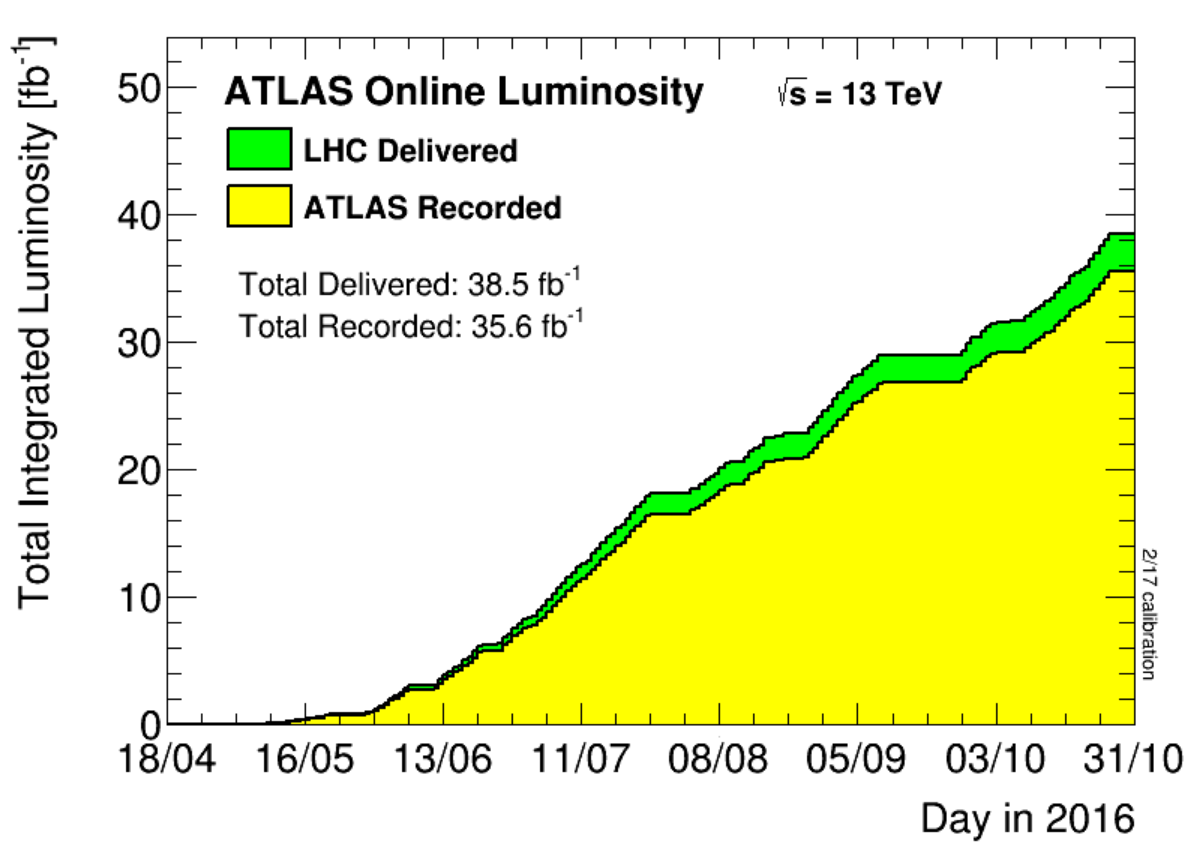
\includegraphics[width=\textwidth]{images/Lumi}
        \caption{Luminosidad acumulada en función del tiempo entregada a (en verde) y registrada por (en amarillo) ATLAS.}
        \label{fig:Lumi}
    \end{subfigure}
    \hfill
    \begin{subfigure}[b]{0.46\textwidth}
        \centering
        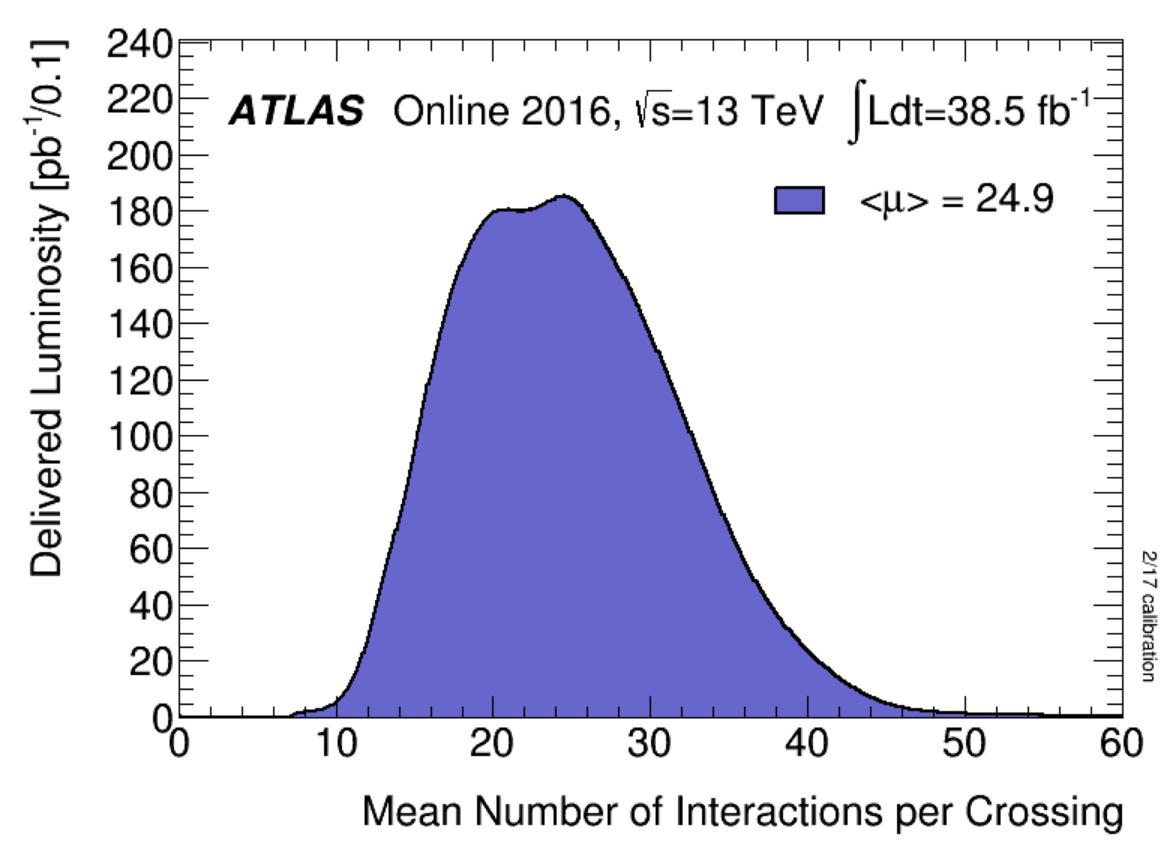
\includegraphics[width=\textwidth]{images/muATLAS}
        \caption{Distribución (pesada por la luminosidad) del número medio de interacciones por bunch crossing.}
        \label{fig:muATLAS}
    \end{subfigure}
    \caption{ Datos correspondientes a colisiones $pp$ a 13 TeV de energía de centro de masa en 2016, desde que el LHC declara tener haces estables hasta que se le informa a ATLAS poner el detector en \emph{stand-by}\cite{LumiATLAS}.}
    \label{fig:Data2016}
\end{figure}

Debido a la alta sección eficaz total inelástica para colisiones $pp$ en el LHC ($\sigma_{pp}\sim\,70mb$) y a la cantidad de protones en un dado paquete, cuando dos paquetes de protones colisionan (``bunch crossing'') en un IP ocurren múltiples interacciones $pp$ en simultáneo. La interacción $pp$ con el momento transverso, $p_t$, más alto en el evento se la conoce como el ``hard scatter'' y todas las colisiones $pp$ adicionales se las conoce como  \emph{pile-up}. Se distinguen dos tipos: \emph{in-time pile-up}, haciendo referencia a aquellas interacciones \emph{pp} en el mismo bunch crossing; y el \emph{out-of-time pile-up} que se origina a partir de interacciones provenientes de otros bunch crossings (muchos de los subsistemas de ATLAS tienen ventanas de medición mayores a 25 ns, que es el intervalo entre bunch-crossings). El número medio de interacciones $pp$ por bunch crossing $<\mu>$ es proporcional a la sección eficaz inelástica total para colisiones $pp$ y a la luminosidad instantánea. Por lo tanto, cambios en la luminosidad según el período de adquisición de datos se traducen en condiciones diferentes de pile-up. En la figura \ref{fig:muATLAS} puede verse la distribución de $<\mu>$ (pesada por la luminosidad) para las colisiones $pp$ a 13TeV durante 2016.

\section{El detector ATLAS}
El experimento ATLAS (\textit{A Toroidal LHC ApparatuS}) en el LHC es un experimento multi-propósito, con simetría aproximadamente cilíndrica, diseñado tanto para hacer mediciones de precisión del SM, como por ejemplo la masa del quark top, parámetros de la violación CP y del Higgs, y la sección eficaz (inclusiva) de producción de jets, como para buscar física más allá del SM, como ser la búsqueda de partículas supersimétricas o materia oscura. En la figura \ref{fig:OverviewATLAS} puede verse un esquema del detector indicando sus dimensiones y sus subsistemas. 

\begin{figure}[H]
    \centering
    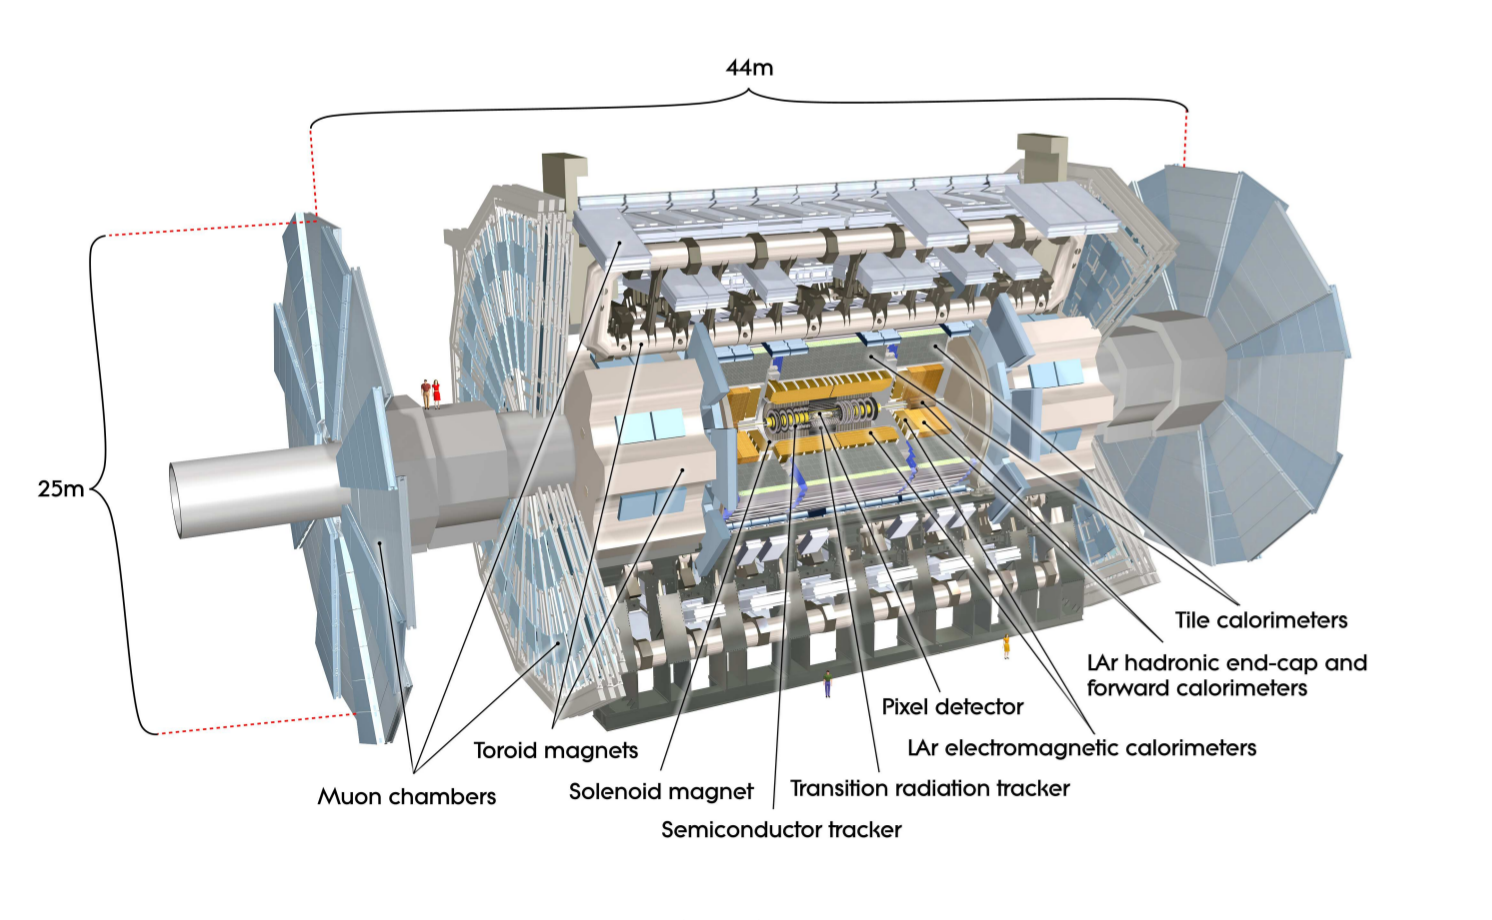
\includegraphics[width =0.8\linewidth]{images/OverviewATLAS}
    \caption{ Esquema del detector ATLAS \cite{OverviewATLAS}.}
    \label{fig:OverviewATLAS}
\end{figure}


\subsection{Sistema de Coordenadas}

El sistema de coordenadas en ATLAS se define con su origen en el centro del detector, dado por el IP. El eje $z$ se elige en la dirección del haz, y el plano $xy$ se toma de manera transversal a este. El eje $x$ se toma sobre la horizontal, con la dirección de los positivos apuntando hacia el centro del anillo del LHC; y la dirección de los $y$ positivos apuntando hacia arriba. En cuanto a las coordenadas cilíndricas, se toma  $\varphi$ alrededor del haz y $\theta$ a partir del eje del haz (ver fig. \ref{fig:sistCoord}).

\begin{figure}[h]
    \centering
    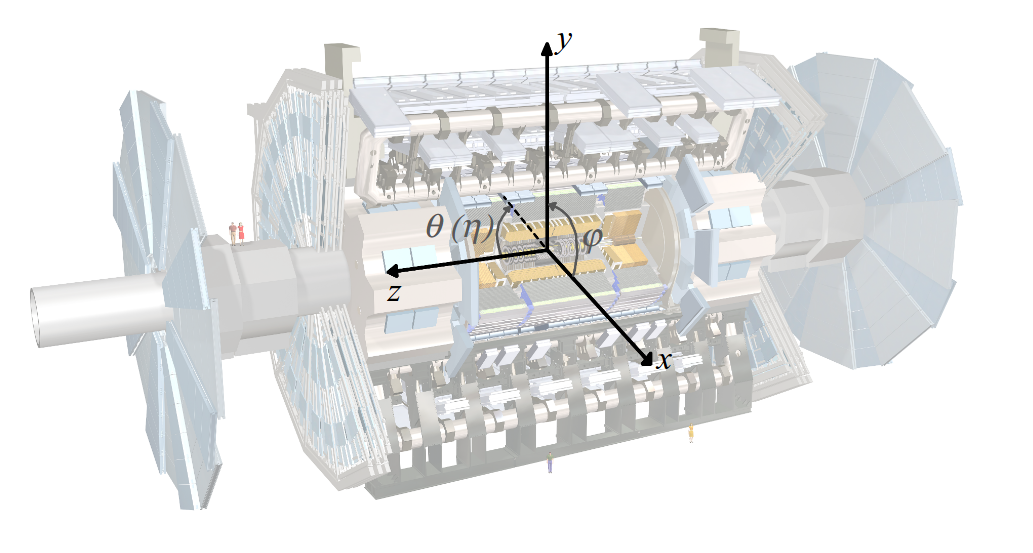
\includegraphics[width =0.5\linewidth]{images/SistCoord}
    \caption{ Sistema de Coordenadas tomado en el experimento ATLAS \cite{OverviewATLAS}.}
    \label{fig:sistCoord}
\end{figure}


Se define la rapidez de una partícula, que resulta una variable invariante de Lorentz,  a partir de su energía ($E$) y su momento longitudinal, es decir la proyección de su momento en la dirección del haz ($p_z$) como:\\
$$ y = \frac{1}{2}\,ln\,\frac{E+p_z}{E-p_z}$$\\
Que las variables resulten invariantes de Lorentz resulta conveniente ya que, en colisiones $pp$, el centro de masa de las colisiones entre partones típicamente se encuentra boosteado respecto del centro de masa $pp$.

En el límite de partículas sin masa, $E>>m$, la rapidez resulta igual a la pseudo-rapidez, dada por: \\
$$ \eta = - ln\, tan\,\frac{\theta}{2} $$ \\
la cual sólo depende del ángulo polar $\theta$, de manera que $\eta=0$ corresponde al plano transverso al haz, y $\eta = \pm\,\infty$ corresponde a la dirección del haz. La distancia angular entre dos objetos medidos en el detector en el plano $(\eta,\varphi)$ está dada por:\\
$$ \Delta\,R=\sqrt{(\Delta\,\eta)^2 + (\Delta\,\varphi)^2} $$

\subsection{Lay-out del detector y sus subsistemas}\label{layout}

La figura  \ref{fig:Event} ejemplifica el paso de diferentes tipos de partículas visto en el plano transverso del detector ATLAS. Las partículas cargadas se identifican haciendo uso de un campo magnético que curva sus trayectorias. Se pueden distinguir electrones y fotones de otras partículas sabiendo que éstos depositan toda su energía en el calorímetro electromagnético, mientras que los hadrones lo hacen en el hadrónico. Por otro lado, se pueden distinguir partículas cargadas de partículas neutras notando que las primeras dejan trazas en el primer tramo del detector. En cuanto a los muones y neutrinos, estos atraviesan enteramente el detector. Sin embargo, mientras que los neutrinos escapan cualquier detección directa, los muones dejan trazas en el espectrómetro de muones. La detección de los neutrinos se dice indirecta ya que sólo se pueden inferir a partir de determinar la energía faltante en una colisión (el momento total en el plano transverso debe ser nulo ya que antes de la colisión los protones viajan sobre el eje del haz).\\

\begin{figure}[h]
    \centering
    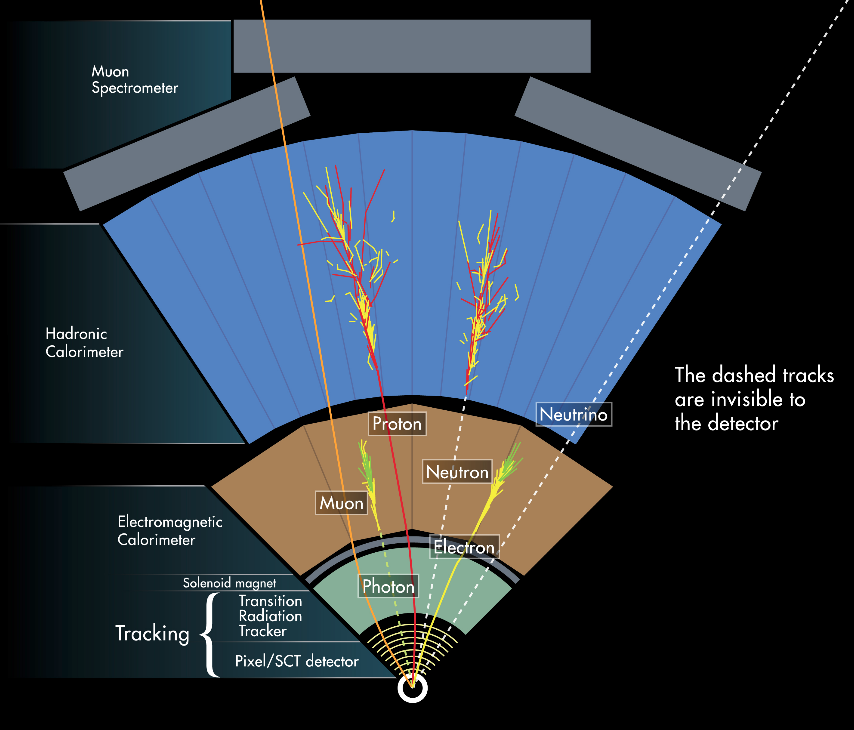
\includegraphics[width =0.9\linewidth]{images/Event}
    \caption{Ilustración de la detección de partículas en el plano transverso del detector ATLAS\cite{Event}}
    \label{fig:Event}
\end{figure}


El detector consiste en un sistema de reconstrucción de trazas o \textit{inner detector (ID)} que cubre un rango de pseudo-rapidez $|\eta|<$2.5, dos calorímetros de sampleo, uno electromagnético y uno hadrónico, que cubren el rango $|\eta|<$4.9, y un espectrómetro de muones que cubre el rango $|\eta|<$2.7. Una descripción detallada de cada uno de ellos puede encontrarse en la referencia \cite{ATLAS}.\\

Desde el IP hacia afuera del detector, el primero de estos subsistemas es el ID. Se utiliza para medir el momento y reconstruir las trazas de las partículas cargadas, y está conformado por tres subdetectores (ver fig \ref{fig:ID}): más próximo al haz se encuentra un detector de píxeles de silicio, seguido de un detector conformado de ``strips'' semiconductoras (SCT o \textit{SemiConductor Tracker}). Ambos siguen el mismo principio de funcionamiento, partículas ionizantes que atraviesan el semiconductor producen pares electrón/hueco que resultan en corrientes que al ser colectadas se interpretan de manera binaria de forma tal que una detección se registra si el pulso medido es mayor a un cierto umbral. El último elemento del ID es un detector de radiación de transición (\textit{Transition Radiaton Tracker} o TRT) que consiste en capas de tubos de 4mm de diámetro, con un cable de tungsteno sobre el eje axial y  un mezcla de gases (xenón, dióxido de carbono y oxígeno) en su interior. De esta manera, al ser atravesados por una partícula cargada, ésta ioniza el gas y se produce una señal eléctrica sobre el cable. Además, partículas relativistas que atraviesan el espacio entre dos tubos (atraviesan diferentes constantes dieléctricas), emiten radiación de transición, lo cual permite distinguir electrones de hadrones cargados (como por ejemplo, piones) ya que a un mismo momento los electrones emiten más fotones que los hadrones. 
Todo el ID a su vez está rodeado de un solenoide que provee de un campo magnético axial (paralelo al haz) de 2T que tuerce la trayectoria de las partículas cargadas permitiendo identificarlas y medir su momento.


Después del Run 1 (primer período de adquisición de datos en ATLAS) se agregó una nueva capa de píxeles de silicio entre el conducto del haz (a 3.3 cm de la línea del haz en dirección radial) y el detector de píxeles anterior llamada ``insertable B-layer'' con el fin de mejorar la identificación de vértices y reconstrucción de trazas, y mejorar la sensibilidad en señales en canales con $b-$jets \cite{IBL}.\\

\begin{figure}[h]
    \centering
    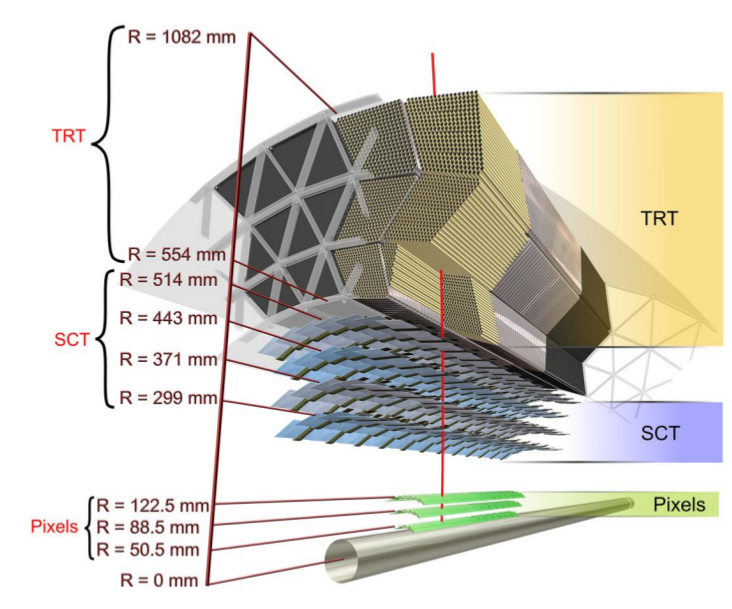
\includegraphics[width =0.6\linewidth]{images/ID}
    \caption{Esquema del \textit{Inner Detector} en ATLAS\cite{ID}.}
    \label{fig:ID}
\end{figure}

El siguiente sistema de detección son los calorímetros, electromagnéticos y hadrónicos, encargados de determinar la energía de las partículas. Los calorímetros se encuentran segmentados en $\eta$ y $\varphi$, aproximadamente simétricos en $\varphi$ pero utilizando diferentes tecnologías para distintos rangos de $\eta$. Cada región del detector tiene al menos tres capas de lecturas calorimétricas que permiten reconstruir el perfil longitudinal de las lluvias.   
El calorímetro electromagnético absorbe y mide la energía de fotones y electrones. También mide la energía de los hadrones, pero éstos no pierden toda su energía en este calorímetro por lo que continúan su paso hasta el calorímetro hadrónico donde se mide su energía restante. 
Los calorímetros de ATLAS son calorímetros de sampleo. Esto quiere decir que contienen dos tipos de material: el absorbente, en el que de las partículas se produce la lluvia y se absorben; intercalado con el material activo, en el que se mide la energía de las partículas producidas en la lluvia. Además, los calorímetros de ATLAS son no-compensadores, es decir, se mide una señal menor para partículas hadrónicas que para partículas electromagnéticas con la misma energía inicial. Como ya se introdujo en la sección \ref{Lluvias}, este efecto tiene que ver con que las interacciones nucleares de los hadrones absorben una cantidad significativa de energía mientras que producen una señal baja, o ninguna, en el calorímetro.\\  

En la figura \ref{fig:Calo} puede observarse la distribución de los distintos calorímetros del experimento ATLAS. Básicamente se utilizan dos tecnologías para el medio activo: calorímetros de argón líquido (LAr) y calorímetros con tejas centelladoras.
Los calorímetros que utilizan LAr como medio activo\footnote{La elección de argón líquido como medio activo se debe a que, al ser un gas noble, garantiza que el camino libre medio de los electrones producidos en la ionización sea mayor que la distancia entre electrodos.} siguen el mismo principio de funcionamiento: una partícula cargada que atraviesa una región con LAr ioniza el líquido y la carga resultante viaja bajo la influencia de una diferencia de potencial hacia los correspondientes electrodos. Los calorímetros-LAr electromagnéticos usan plomo como absorbente y cubren la región central $|\eta|<$1.475 (`` barrel'') y las tapas cilíndricas 1.375$<|\eta|<$3.2 (``end-caps''), con un grosor total mayor a 22 $X_0$ en el barrel  y mayor a 24 $X_0$ en los end-caps; y los hadrónicos usan cobre como material absorbente y están ubicados en la región end-cap (1.5$<|\eta|<$3.2). Los calorímetros en la región delantera o ``forward'' (FCal), 3.1$<|\eta|<$4.9, también usan LAr como medio activo, y cobre (electromagnético) o tungsteno (hadrónico) como material absorbente. A continuación se encuentran los calorímetros hadrónicos de tejas (o ``Tile''): en el barril central cubriendo la región $|\eta|<$1.0, y dos barriles extendidos en la región 0.8$<|\eta|<$1.7, los cuales usan tejas centelladoras como material activo y placas de acero como material absorbente. El principio de detección en este caso se basa en colectar la luz centelleante producida por partículas ionizantes en el material activo utilizando una fibra óptica, y transformar esta señal en una señal eléctrica usando fotomultiplicadores. Los calorímetros hadrónicos tienen un grosor aproximado de 7.4 $\lambda$ en el barrel y 10 $\lambda$ en la región end-cap, minimizando la cantidad de hadrones que pudieran llegar al espectrómetro de muones. \\

\begin{figure}[h]
    \centering
    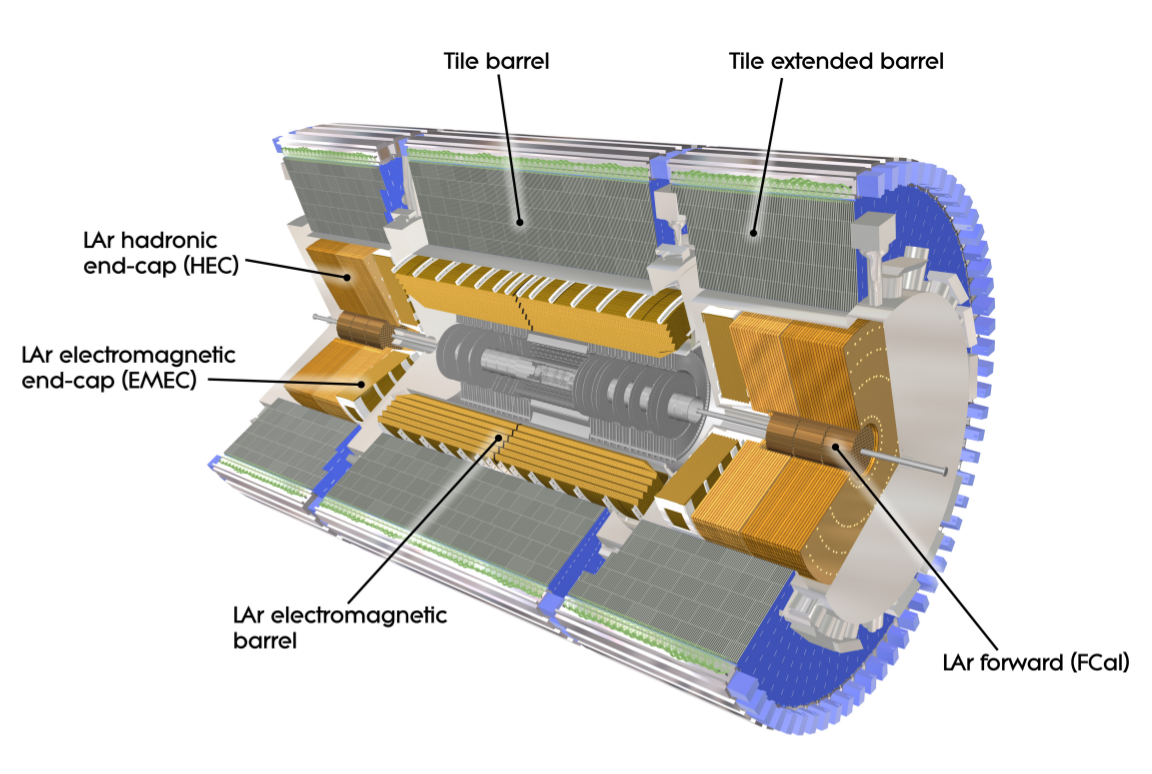
\includegraphics[width =0.7\linewidth]{images/Calo}
    \caption{Esquema del sistema de Calorímetros en ATLAS \cite{Calo}.}
    \label{fig:Calo}
\end{figure}

Por último, en la parte más exterior de ATLAS, se encuentra el espectrómetro de muones (MS), diseñado para detectar las partículas cargadas (muones\footnote{Los muones son partículas poco ionizantes para los valores de momento relevantes en ATLAS y por lo tanto no son absorbidos por los calorímetros.} o partículas de modelos más-allá del SM) que logran atravesar los calorímetros, midiendo su momento en el rango $|\eta|<$2.7 y brindando una decisión de trigger sobre ésta partícula en el rango $|\eta|<$2.4. El MS se basa en la deflexión de las trazas de los muones ocasionada por un sistema de toroides magnéticos sin núcleo (para minimizar la cantidad de material atravesado por los muones al salir de los calorímetros).
El MS cuenta con cámaras de rastreo de precisión y cámaras de trigger. El lay-out del MS puede verse en la figura \ref{fig:MS}.
\begin{figure}[h]
    \centering
    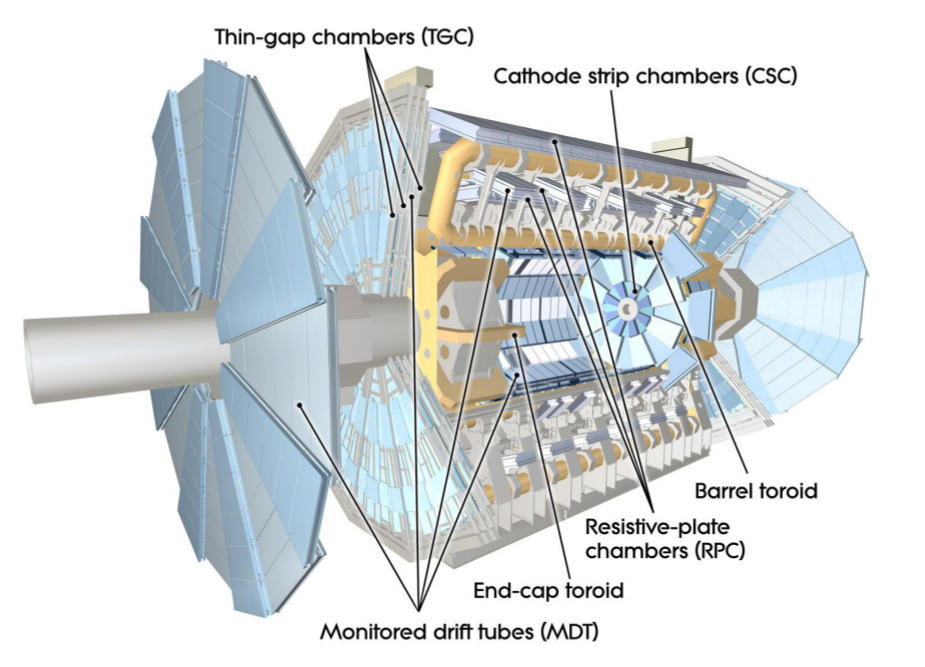
\includegraphics[width =0.7\linewidth]{images/MS}
    \caption{Esquema del sistema del espectrómetro de muones en ATLAS \cite{MS}.}
    \label{fig:MS}
\end{figure}

Dos tecnologías se utilizan para las cámaras de rastreo: tubos de deriva o \textit{Monitored Drift tubes} (MDT) y \textit{Cathode Strip Chambers} (CSC). Las cámaras MDT consisten de varias capas de tubos de aluminio de 3cm de diámetro, llenos de una mezcla de gases (Ar y CO$_2$) con un cable en el centro que actúa como ánodo. De esta manera, una partícula cargada que atraviesa este sistema, ioniza el gas, y se mide el tiempo que tardan los iones en viajar hacia el ánodo. Los MDTs cubren un rango de hasta $|\eta|<$2.7, excepto en la primera capa en los end-caps donde cubren un rango $|\eta|<$2.0. Los CSC son cámaras multi-cable que siguen el mismo principio de funcionamiento que los MDTs, pero incorporan dos tipos de cátodos en ``strips'' orientadas perpendicularmente entre si, permitiendo la medición tanto en la dirección $\eta$ como en $\varphi$; y cubren la primera capa en los end-caps en el rango 2.0$<|\eta|<$2.7 donde se necesita una resolución mayor. 

Las cámaras de trigger están diseñadas para identificar el bunch-crossing, activar el trigger sobre muones y medir la segunda coordenada de la traza del muón en la dirección ortogonal a la determinada por las cámaras MDT. Este sistema está compuesto por las cámaras de placas resistivas (RPC) y por las cámaras \textit{thin-gap} (TGC). Las RPC se encuentran en el barril y cubren la región $|\eta|<$1.05. Consisten de dos placas paralelas resistivas separadas una distancia de 2mm. En el gap se introduce una mezcla de gases de manera tal que un muón que atraviesa el gas induce una avalancha hacia el ánodo. Las TGC son cámaras multi-cable ubicadas en la región end-cap (1.05$<|\eta|<$2.4), con la característica de que la distancia cable/cátodo es menor a la distancia cable/cable, asegurando un tiempo de deriva menor a los 25ns que corresponde al intervalo entre bunches. 

\subsubsection{Reconstrucción de Muones}\label{Muones}

En general, los muones en ATLAS se reconstruyen independientemente en el ID y en el MS para luego combinar la información individual de los sub-detectores de manera de formar las trazas de muones que luego serán utilizadas en los análisis físicos. El ID provee la mejor medición a bajo momento ($>$3GeV), mientras que el MS lo hace para $p_t>$30GeV (y hasta aproximadamente 3TeV). Se definen distintos tipos de muones según los sub-detectores usados en su reconstrucción. Un detalle de la reconstrucción de muones y de los distintos tipos de muones definidos puede encontrarse en la referencia \cite{MuonReco}.

En las simulaciones de MC, el momento de los muones debe ser corregido para llevar la escala y resolución de momento de muones en MC a la observada en datos \cite{MuonCalib}.  

Los muones utilizados en este estudio son \textit{Combined Muons}. En este caso, la reconstrucción de su traza se realiza de manera independiente en el ID y en el MS, y se forma una traza combinada a partir de un ajuste global que usa los hits en ambos subdetectores. Durante este procedimiento pueden agregarse o removerse hits en el MS de manera de mejorar la calidad del ajuste. La mayoría de los muones se reconstruyen siguiendo una estrategia de tipo ``afuera-hacia-adentro'' en la que los muones primero se reconstruyen en el MS y luego se extrapolan hacia el interior del detector identificándolos con trazas en el ID. La estrategia inversa, en la que las trazas en el ID se extrapolan hacia afuera y se identifican con trazas en el MS, se usa como enfoque complementario. La reconstrucción de los combined muons está limitada por la aceptancia del ID ($|\eta|<$2.5). 
%estos al final creo que no lo pongo.
%En el caso de los Muones extrapolados, la trayectoria del muón se reconstruye utilizando únicamente la traza en el MS, pidiendo una ``leve'' compatibilidad con el IP. Los parámetros de la traza del muón en este caso se definen en el IP, considerando la pérdida de energía estimada en los calorímetros. En general también se pide que el muón haya atravesado dos capaz de cámaras en el MS (o tres si se trata de la región delantera) para generar 

Una vez reconstruidos los muones, se los cataloga según distintos criterios de calidad en \textit{Tight, Medium, Loose y High-p$_t$}\footnote{Las categorías \textit{Tight, Medium y Loose} son inclusivas en el sentido de que la categoría Medium incluye a la Tight, y la Loose incluye a las otras dos.} con el fin de satisfacer las necesidades de diferentes análisis físicos\cite{MuonReco}. En general, para garantizar una buena medición del momento, se requiere un número específico de hits en el ID y MS. Para el ID se pide que haya al menos un hit en el detector de píxeles, al menos cinco en el SCT y menos de tres agujeros\footnote{Un agujero se define como un sensor activo que es atravesado por la traza pero en el que no se observan hits. Un faltante de hit sólo se considera agujero cuando cae entre hits que fueron asignados exitosamente a una dada traza.} en cualquiera de los dos. Para la región 0.1$<|\eta|<$0.9 (región de aceptancia del TRT) además se pide que al menos el 10$\%$ de los hits en el TRT que se asignaron inicialmente a la traza estén incluidos en el ajuste final. 

En esta tesis se seleccionan sólo los muones que satisfacen el criterio ``Medium'', selección por default para los muones en ATLAS. Esta selección minimiza la incerteza sistemática asociada a la reconstrucción y calibración de los muones. Este criterio pide a los Combined Muons que tengan al menos tres hits en al menos dos capas de cámaras MDT en el MS; excepto para trazas en la región $|\eta|<$0.1 donde se pide que la traza tenga al menos un hit en alguna capa MDT pero no más de un agujero en alguna capa MDT. Además, se pone un corte en la significancia\footnote{La significancia $q/p$ se define como el valor absoluto de la diferencia entre el cociente carga/momento del muón en el ID y en el MS, dividido por la suma en cuadratura de sus incertezas correspondientes.} $q/p$ de manera de suprimir la contaminación que surge de identificar incorrectamente hadrones como muones. 

Los muones que se originan como resultado del decaimiento de partículas pesadas, como el Z, generalmente se producen aislados de otras partículas, a diferencia de los muones que se producen en decaimientos semi-leptónicos, los cuales se encuentran envueltos en jets. Por lo tanto, otro corte referido a la calidad de los muones considerados tiene que ver con la aislación. Se definen distintos criterios de aislación, cada uno optimizado para distintos análisis, teniendo en cuenta variables relacionadas con las trazas o con la energía depositada en celdas calorimétricas en conos de diferentes $\Delta R$. 


\subsection{Trigger y Adquisición de Datos}

La cantidad de información que se produce en el detector ATLAS supera enormemente la cantidad que puede ser almacenada y analizada. El sistema de Trigger y Adquisición de Datos (TDAQ) tiene la tarea de reducir la frecuencia de adquisición de eventos sin perder los eventos de ``interés''. Básicamente, el \textit{trigger} busca eventos que contienen objetos con alto $p_t$, como por ejemplo clusters electromagnéticos, jets y taus, o eventos con un gran faltante de momento transverso.
El trigger se conforma de dos niveles, el \textit{nivel-1} o L1 basado en hardware, seguido por el \textit{high-level-trigger} o HLT basado en software.
El L1 reduce la frecuencia de eventos desde los $\sim40MHz$ dado por la frecuencia de colisión de los paquetes de protones a una frecuencia del orden de $\sim100kHz$ con una latencia de 2.5$\mu\,s$. El L1 define regiones de interés (RoI) en el plano ($\eta,\varphi$): una región del detector en donde se midió un valor grande de $E_t$, energía depositada en el calorímetro, o en donde se midió una traza de alto momento en el sistema de muones. Si el L1 efectivamente encuentra una RoI, entonces se dice que pasa al nivel HLT. En el HLT, se corren algoritmos rápidos de reconstrucción, como los usados a nivel \textit{offline} (ver sección \ref{JetAlgo}), sobre las RoI halladas por el L1 que toman una decisión en menos de 300 ms. 
Los eventos que fueron aceptados por el HLT se escriben en distintos \textit{streams} de datos, a una frecuencia promedio de $1kHz$, para usarse ya sea en análisis de física o de trigger, o realizar monitoreos o calibraciones del detector. 
%Dependiendo del \textit{stream} se guarda la información completa del evento (por ejemplo para realizar análisis físicos), o sólamente una parte de ella (por ejemplo para análisis del trigger, monitoreos o calibrar el detector).
Para reducir la adquisición de cierto tipo de eventos que, si bien son de interés, tienen una sección eficaz alta, algunos triggers también se encuentran \textit{pre-escaleados}. Es decir, para un trigger con pre-escaleo de $N$, uno de cada $N$ eventos que disparan ese trigger se selecciona para ser almacenado. La decisión de qué triggers pre-escalear y con qué factor se toma teniendo en cuenta la luminosidad instantánea entregada al detector y cuáles objetos son los más demandados para realizar análisis físicos \cite{Trigger}. 


